\section{Марериалы работы}
\subsection{Экспериметральная установка}
\begin{figure}[!h]
    \centering
    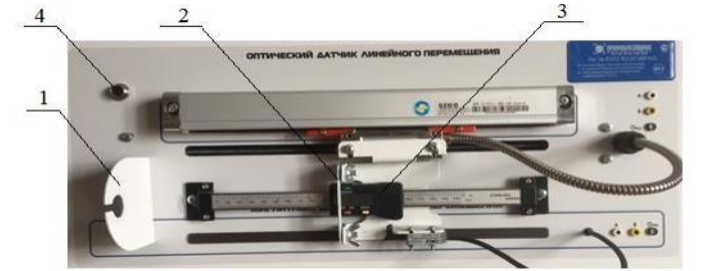
\includegraphics[width=0.9\textwidth]{img/img}
    \caption{Зона испытание бесконтактных датчиков}
    \label{fig:img}
\end{figure}
\begin{enumerate}
    \item Неподвижная стойка
    \item Передвижной механизм крепления
    \item Измерительное устройство
    \item Разъем для подключения датчика
\end{enumerate}
\subsection{Исследование датчиков}
В эксперименте участвуют пять датчиков:
\begin{itemize}
    \item OV A43A-31P-150-LZ (оптический)
    \item ISN EF41A-31P-8-LZ (индуктивный)
    \item CSN E41A5-31P-10-LZ (емкостной)
    \item MS BO3A-L (геркон)
    \item Ультразвуковой датчик
\end{itemize}

Проведем исследование, определяя расстояние срабатывания и отпускания датчиков при использовании различных материалов в качестве препятствия.
Результаты измерений занесем в соответствующие таблицы.
\begin{table}[!h]
    \centering
    \caption{Показания оптического датчика OV A43A-31P-150-LZ}
    \label{tab:1}
    \begin{tabular}{|c|c|c|c|c|c|c|c|c|c|c|c|c|}
        \hline
        & \multicolumn{6}{c|}{Расстояние срабатывания, мм} & \multicolumn{6}{c|}{Расстояние отпускания, мм}\\
        \cline{2-13}
        \raisebox{1.5ex}[0cm][0cm]{Материал мишени}
        & 1 & 2&3 &4 &5 & Среднее &1 &2 &3 &4 &5 &Среднее \\
        \hline
        Желтый пластик & 0 & 0 & 0 & 0 & 0 & 0 & 195 & 193 & 197 & 189 &186 & 192\\
        Черный пластик & 0 & 0 & 0 & 0 & 0 & 0 & 173 & 176 & 172 & 172 &173 & 173.2\\
        Оргстекло & 0 & 0 & 0 & 0 & 0 & 0 & 179 & 175 & 176 & 175 &178 &176.6\\
        Металл & 0 & 0 & 0 & 0 & 0 & 0 & 51 & 53 & 59 & 45 &48 & 51.2\\
        \hline
    \end{tabular}
\end{table}
\begin{table}[!h]
    \centering
    \caption{Показания индуктивного датчик ISN EF41A-31P-8-LZ}
    \label{tab:2}
    \begin{tabular}{|c|c|c|c|c|c|c|c|c|c|c|c|c|}
        \hline
        & \multicolumn{6}{c|}{Расстояние срабатывания, мм} & \multicolumn{6}{c|}{Расстояние отпускания, мм}\\
        \cline{2-13}
        \raisebox{1.5ex}[0cm][0cm]{Материал мишени}
        & 1 & 2&3 &4 &5 & Среднее &1 &2 &3 &4 &5 &Среднее \\
        \hline
        Желтый пластик & -& -& -& -& -& -& -& -& -& -& -& -\\
        Черный пластик& -& -& -& -& -& -& -& -& -& -& -& -\\
        Оргстекло & -& -& -& -& -& -& -& -& -& -& -& -\\
        Металл & 0 & 0 & 0 & 0 & 0 & 0 & 36 & 35 & 36 & 35 &36 & 35.6\\
        \hline
    \end{tabular}
\end{table}

\begin{table}[!h]
    \centering
    \caption{Показания емкостного датчик CSN E41A5-31P-10-LZ}
    \label{tab:3}
    \begin{tabular}{|c|c|c|c|c|c|c|c|c|c|c|c|c|}
        \hline
        & \multicolumn{6}{c|}{Расстояние срабатывания, мм} & \multicolumn{6}{c|}{Расстояние отпускания, мм}\\
        \cline{2-13}
        \raisebox{1.5ex}[0cm][0cm]{Материал мишени}
        & 1 & 2&3 &4 &5 & Среднее &1 &2 &3 &4 &5 &Среднее \\
        \hline
        Желтый пластик & 0& 0& 0& 0& 0& 0& 31& 32& 31& 32& 31& 31.3\\
        Черный пластик& 0& 0& 0& 0& 0& 0& 31& 32& 31& 31& 32& 31.6\\
        Оргстекло & 0& 0& 0& 0& 0& 0& 31& 31& 31& 31& 31& 31\\
        Металл & 0 & 0 & 0 & 0 & 0 & 0 & 36 & 36 & 35 & 37 &36 & 36\\
        \hline
    \end{tabular}
\end{table}

\begin{table}[!h]
    \centering
    \caption{Показания геркона MS BO3A-L}
    \label{tab:4}
    \begin{tabular}{|c|c|c|c|c|c|c|c|c|c|c|c|c|}
        \hline
        & \multicolumn{6}{c|}{Расстояние срабатывания, мм} & \multicolumn{6}{c|}{Расстояние отпускания, мм}\\
        \cline{2-13}
        \raisebox{1.5ex}[0cm][0cm]{Материал мишени}
        & 1 & 2&3 &4 &5 & Среднее &1 &2 &3 &4 &5 &Среднее \\
        \hline
        Желтый пластик & -& -& -& -& -& -& -& -& -& -& -& -\\
        Черный пластик& -& -& -& -& -& -& -& -& -& -& -& -\\
        Оргстекло & -& -& -& -& -& -& -& -& -& -& -& -\\
        Металл & -& -& -& -& -& -& -& -& -& -& -& -\\
        Магнит & 0 & 0 & 0 & 0 & 0 & 0 & 3 & 4 & 3 & 4 &3 & 3.33\\
        \hline
    \end{tabular}
\end{table}

\begin{table}[!h]
    \centering
    \caption{Показания ультразвукового датчика расстояния}
    \label{tab:5}
    \begin{tabular}{|c|c|c|c|c|c|c|c|c|c|c|c|c|}
        \hline
        & \multicolumn{6}{c|}{Расстояние срабатывания, мм} & \multicolumn{6}{c|}{Расстояние отпускания, мм}\\
        \cline{2-13}
        \raisebox{1.5ex}[0cm][0cm]{Материал мишени}
        & 1 & 2&3 &4 &5 & Среднее &1 &2 &3 &4 &5 &Среднее \\
        \hline
        Желтый пластик & 110&  108& 105& 95& 108& 105.2& 775& 675& 645& 655& 608& 671.6\\
        Черный пластик& 115& 110& 115& 195& 175& 142& 665& 675& 695& 772& 740& 709.4\\
        Оргстекло & 115& 145& 145& 107& 110& 124.4& 705& 734& 734& 725& 778& 735.2\\
        Металл & 45& 55& 67& 73& 69& 61.8& 68& 67& 66& 68.5& 69& 67.75\\
        \hline
    \end{tabular}
\end{table}

\section{Вывод}
В ходе работы были проведены испытания бесконтактных датчиков приближения и определены их нижние и верхние границы срабатывания при использовании различных материалов в качестве препятствия.

Границы срабатывания оптического датчика зависят от светоотражающих свойств поверхности,
индуктивный датчик сработал только при использовании металлической пластины в качестве поверхности, геркон -- только при использовании магнита, а емкостной датчик сработал при использовании в качестве препятствия всех доступных вариантов материалов.

При исследовании ультразвукового установлено, что расстояние отпускания для металлической пластины на порядок меньше, чем для других материалов.
Это связано с тем, что металлическая пластина имела меньший размер по сравнению с другими, что не давало возможности датчику корректно зафиксировать ее присутствие.